\documentclass[12pt, openany]{report}
\usepackage[utf8]{inputenc}
\usepackage[T1]{fontenc}
\usepackage[a4paper,left=2cm,right=2cm,top=1cm,bottom=2cm]{geometry}
\usepackage[french]{babel}
\usepackage{libertine}
\usepackage[pdftex]{graphicx}
\usepackage[export]{adjustbox}
\usepackage{setspace}
\usepackage{hyperref}
\usepackage{enumitem}
\usepackage[nottoc]{tocbibind}
\usepackage{amsmath,diagbox,tabu}
\usepackage{caption}
\usepackage{float}

\hypersetup{
    colorlinks=true,
    linkcolor=black,
    filecolor=magenta,      
    urlcolor=cyan,
}
\setstretch{1,4}
\setlength{\parindent}{4ex}
\setlength{\parskip}{1ex plus 0.5ex minus 0.2ex}
\newcommand{\hsp}{\hspace{20pt}}
\newcommand{\HRule}{\rule{\linewidth}{0.5mm}}

\newlist{mylist}{itemize}{3}
\setlist[mylist,1]{
    label=\textbullet,
    wide=0pt,
    itemindent=\dimexpr\parindent+\labelwidth+\labelsep\relax}

\begin{document}
\begin{titlepage}
  \begin{sffamily}
  \begin{center}

	\begin{figure}[t]
	   \begin{minipage}{0.48\textwidth } 
	     
\includegraphics[width=.3\linewidth , left]{ensias.JPG}
	   \end{minipage}\hfill
	   \begin{minipage}{0.48\textwidth }
	     
\includegraphics[width=.4\linewidth , right]{univesite.JPG}
	   \end{minipage}
	\end{figure}
     
    \textsc{\LARGE École nationale supérieure d'informatique et d'analyse des systèmes}\\[4cm]


    % Title
    \HRule \\[0.5cm]
    { \huge \bfseries Présentation du sujet de projet de fin d'année: Crop Mapping\\[0.4cm] }
	\HRule\\[4cm]

    % Author and supervisor
    \begin{minipage}{0.4\textwidth}
      \begin{flushleft} \large
        \emph{Réalisé par:}\\
            AIT LAHCEN \textsc{Ahmed}\\
	        CHICHI \textsc{Hamza}\\
       \emph{Filière, Groupe}\\
	        Génie logiciel, GL 1\\
      \end{flushleft}
    \end{minipage}
    \begin{minipage}{0.4\textwidth}
      \begin{flushright} \large
       \emph{Sous la direction de:}\\
	Mme. Sanaa. \textsc{EL FKIHI}\\
	\end{flushright}
    \end{minipage}

    \vfill

    % Bottom of the page
    {\large Année universitaire 2019/2020}

  \end{center}
  \end{sffamily}
\end{titlepage}
\newpage
\strut 


\listoffigures
\tableofcontents
\chapter*{Introduction générale}
\addcontentsline{toc}{chapter}{Introduction générale}

Le domaine de l’agriculture constitue une grande partie économique de plusieurs pays dans le monde, ce qui rend la recherche scientifique envers ce secteur d’activité une importante source de revenue financier, mais ceci n’est possible que si la disponibilité des ressources de l’environnement biophysique et humain est importante.
\par
En effet, l’exploitation des images satellites sur les terrains agricoles permet de gérer plus efficacement les récoltes et de prévoir les risques pouvant menacer la production comme par exemple les risques d’infestations d’insectes, les intempéries, la sécheresse ... Et ceci grâce aux différents caractéristiques contenues dans une image satellitaire (longueurs d’ondes, fréquences, domaines spéctraux..)
\par
Si l’agriculture représente un secteur économique très important pour un pays, comme le Maroc par exemple, vaut mieux investir dans la recherche de nouvelles technologies dans ce domaine afin d’exploiter au maximum ses ressources, sans oublier que le développement de l’agriculture moderne ne cesse d’accroitre et que certains pays se sont mis à l’introduction dans les pratiques agricoles de nouveaux outils numériques d’aide à la décision basés sur le monde de la big data et des nouvelles technologies (drones, robots…).
\par
Parmi les technologies modernes qui facilitent la tâche pour les acteurs de la production et augmente la consommation	 agricole, on retrouve le \textbf{Crop Mapping}, qui est le sujet de notre projet de fin d’année.  Cette dernière est une techniques qui utilise des données fournies par les image satellites pour les analysées et les traitées en utilisant plusieurs méthodes telles que le Deep Learning et le réseaux de neurones afin d’élaborer des stratégies pour les champs et les cultures pour le long terme.
\par
Ce rapport est constitué en deux parties. La première partie, intitulée contexte générale du projet, comporte ... chapitres, le premier présente les notions générales du sujets.


\part{Étude du sujet}
Cette partie va présenter les différentes notions abordées dans le projet accompagnées de quelques exemples. 

\chapter{Présentation du sujet}
\section{Les parcelles}

\subsection{Définition de parcelle}
Une parcelle est généralement une superficie de terrain ayant une unité de propriété, elle peut être dans ce cas la propriété privée ou publique d'une personne ou d'un groupe.\\
Un ensemble de parcelles peut être désigné comme un « parcellaire ». 

\begin{figure}[hp]
\centering
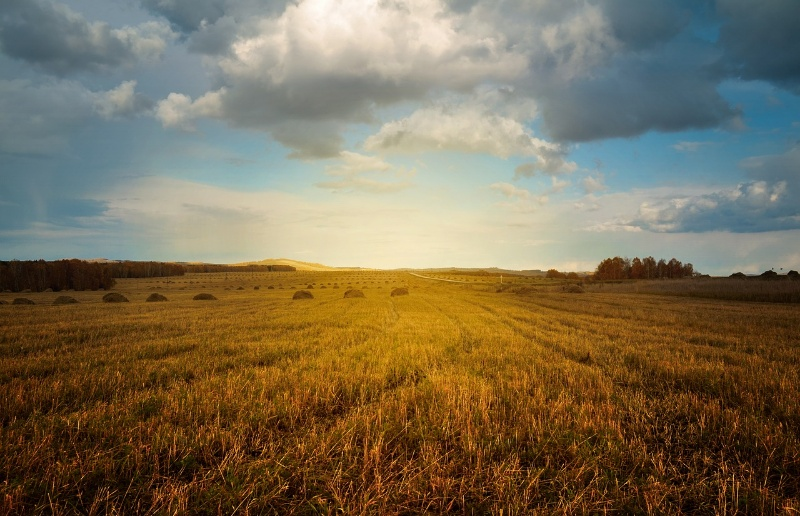
\includegraphics[scale=0.4]{parcelle2.jpg}
\caption{Une parcelle}
\end{figure}


Le terme de parcelle peut s'appliquer à différents domaine :

\begin{mylist}

\item En agriculture, elle désigne la division agricole (champ, pré, vignoble, verger, etc.) exploitée par la même personne ou le même groupe de personnes.


\item En urbanisme, elles sont définies selon leurs propriétaires et leurs limites, tant en milieu rural qu'urbain. Ainsi elle peut être un terrain habité, ou encore une parcelle à l'abandon ou bien une zone de stationnements automobiles. 

\end{mylist}



\subsection{La segmentation des parcelles}

La fragmentation spatiale des parcelles agricoles a un fort impact sur les flux d’eau dans les paysages cultivés, et pour surveiller les paysages à grandes échelles, il y a un fort besoin de délimitation automatique ou semi-automatique des parcelles agricoles. C’est pour cela que la contribution des images satellitaires à très haute résolution peut permettre la délimitation en utilisant de nombreuses méthodes de classification et des algorithmes qui traitent les caractéristiques de ces images.\cite{frag}

\begin{figure}[hp]
\centering
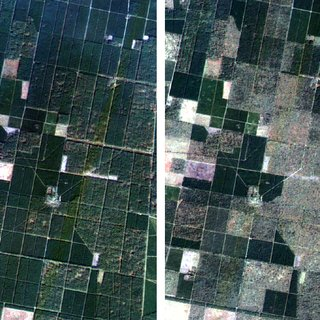
\includegraphics[scale=1]{seg.jpg}
\caption{La fragmentation d'une parcelle}
\end{figure}

Le résultat de ces études permet une bonne localisation des limites parcellaires et met en évidence l’intérêt d’un modèle global si une base de données d’images de limites parcellaires existe. 

\newpage

\subsection{L'agriculture au Maroc}

L'agriculture est un secteur économique très important du Maroc. Il génère environ 14 \% du produit intérieur brut (PIB), mais avec des variations importantes (11 à 18 \%) selon les années en fonction des conditions climatiques. Ses performances conditionnent même celles de l’économie tout entière : le taux de croissance du pays est fortement corrélé à celui de la production agricole. L’agriculture demeure par ailleurs le premier pourvoyeur d’emplois du pays, loin devant les autres secteurs économiques, 40 \% de la population active vivant de ce secteur.\cite{imagesatt}

L’agro-industrie marocaine dont de nombreuses composantes jouissent de certifications ISO peut, légitimement être fière de tout le progrès accompli. Son savoir-faire confirmé lui permet de se placer sur de nombreux marchés extérieurs, très exigeants en qualité, avec des produits très diversifiés relevant de 10 classes différentes.\cite{agr}


\begin{figure}[hp]
\centering
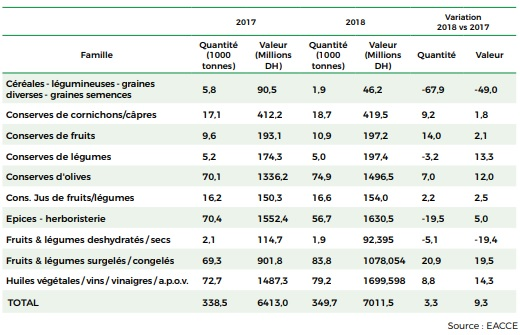
\includegraphics[scale=0.9]{agr.jpg}
\caption{L'agro-industrie au maroc entre 2017 et 2018}
\end{figure}


Les principales productions végétales du pays sont constituées par les céréales (blé, orge), les agrumes (oranges, clémentines), les olives, les rosacées fruitières (amandes, pommes, abricots...), les betteraves à sucre, les légumineuses alimentaires, les cultures maraichères dont les pommes de terre et les tomates, fer de lance des exportations agricoles marocaines. L'élevage (ovin, caprin, bovin, camelin, avicole) constitue aussi une composante importante du secteur agricole en contribuant à hauteur de 30 \% à sa valeur ajoutée.

\section{Les images satellites}
Un satellite artificiel est un objet fabriqué par l'être humain, envoyé dans l'espace à l'aide d'un lanceur et gravitant autour d'une planète ou d'un satellite naturel comme la Lune.  
Le premier satellite artificiel Spoutnik 1 est lancé par l’Union des républiques socialistes soviétiques en 1957.
\subsection{Les sattelites en orbite autour de la terre}


Selon l'association UCS (Union of Concerned Scientists), 2.063 satellites opérationnels étaient en orbite autour de la Terre au 1er avril 2019. Le plus ancien encore en opération est un satellite amateur américain, Amsat-Oscar 7 (AO-7), lancé le 15 novembre 1974. La cadence des lancements s'est brusquement accélérée ces dernières années, avec 378 satellites lancés en 2017 et 375 satellites en 2018. Attention : il ne s'agit pas du nombre de fusées, car les lancements multiples sont devenus la norme. Le 15 février 2017, l'Inde a ainsi battu un record avec 104 satellites en un seul tir.\cite{orbite}

\begin{figure}[hp]
\centering
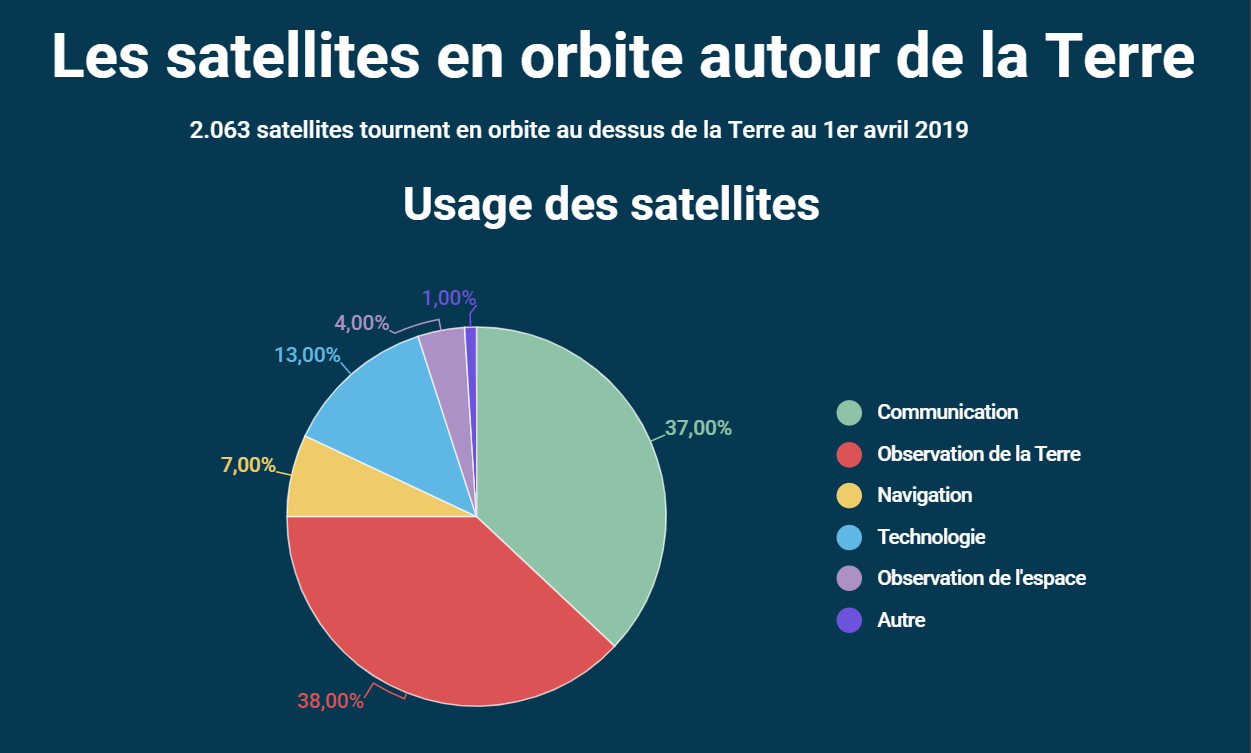
\includegraphics[scale=0.6]{satellite.png}
\caption{Statistiques de satellites}
\end{figure}

\subsection{Les satellites marocains}
Mohammed VI est un système de 2 satellites de reconnaissance et d'observation de la Terre (A et B) du type Pléiades, conçu par Thales Alenia Space (conception de la charge) et Airbus (conception de la plate-forme satellitaire) pour le compte du Centre royal de télédétection spatiale (Maroc).
\par
Le satellite Mohammed VI A est lancé le 8 novembre 2017 par un lanceur Vega depuis le Centre spatial de Kourou satellite espion, il est utilisé pour surveiller le Front Polisario dans la « zone tampon ».
Le lancement du deuxième satellite (Mohammed VI B) est effectué avec succès le 21 novembre 2018, à usage civil, est utilisé pour la cartographie et le cadastre, l’identification des zones sinistrées...
\begin{figure}[h]
\centering
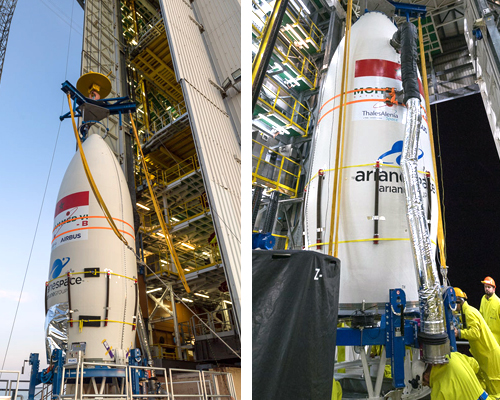
\includegraphics[scale=0.8]{satm6.jpg}
\caption{Le satellite MOHAMMED VI - B}
\end{figure}


\subsection{La définition d'une image satellite}
Une image satellite, ou image satellitaire, est une prise de vue transmise d'un satellite artificiel en orbite. Elles permettent d'obtenir différentes informations comme la surveillance des pays ennemis pour les militaires (fonction première de la création d'un satellite d'observation), prévisions météorologiques (par exemple les satellites Météosat), ou tout simplement pour les recherches sur l'Univers. Certains satellites sont capables d'une précision telle que cela peut devenir un problème, notamment en termes de vie privée ou de secret d'État. 

\subsection{Les caractéristiques des images satellites}
La principale différence entre une photographie et une image satellite est que la photographie est au format analogique et qu’elle est généralement imprimée sur papier avant d’être interprétée. L’image satellite est au format numérique et elle est généralement analysée et interprétée à l’aide d’un ordinateur.Le format numérique enregistre chaque bloc d’informations de manière discrète.


\par
\underline{Le pixel :}
\par

Avec un zoom avant suffisant sur une image satellite, on peut voir de nombreux carrés de couleurs différentes qui sont les pixels.
Ces pixels représente la plus petite unité figurant sur une image. Réunis, ils fournissent toute l’information qui constitue l’image dans son intégralité.

\par
\underline{La résolution spatiale :}
\par 

La résolution spatiale d’une image est la plus petite distance entre deux objets adjacents que le capteur puisse identifier.
Plus les pixels seront nombreux dans l’image plus la résolution spatiale sera élevée.
\par
Selon les caractéristiques du capteur, l’altitude du satellite ,son orbite autour de la Terre, les images satellites seront composées de pixels couvrant une surface au sol plus ou moins grande du sol. On classera ainsi les images enregistrées en images : Basse , moyenne, haute résolution ou très haute résolution.

\begin{figure}[h]
\centering
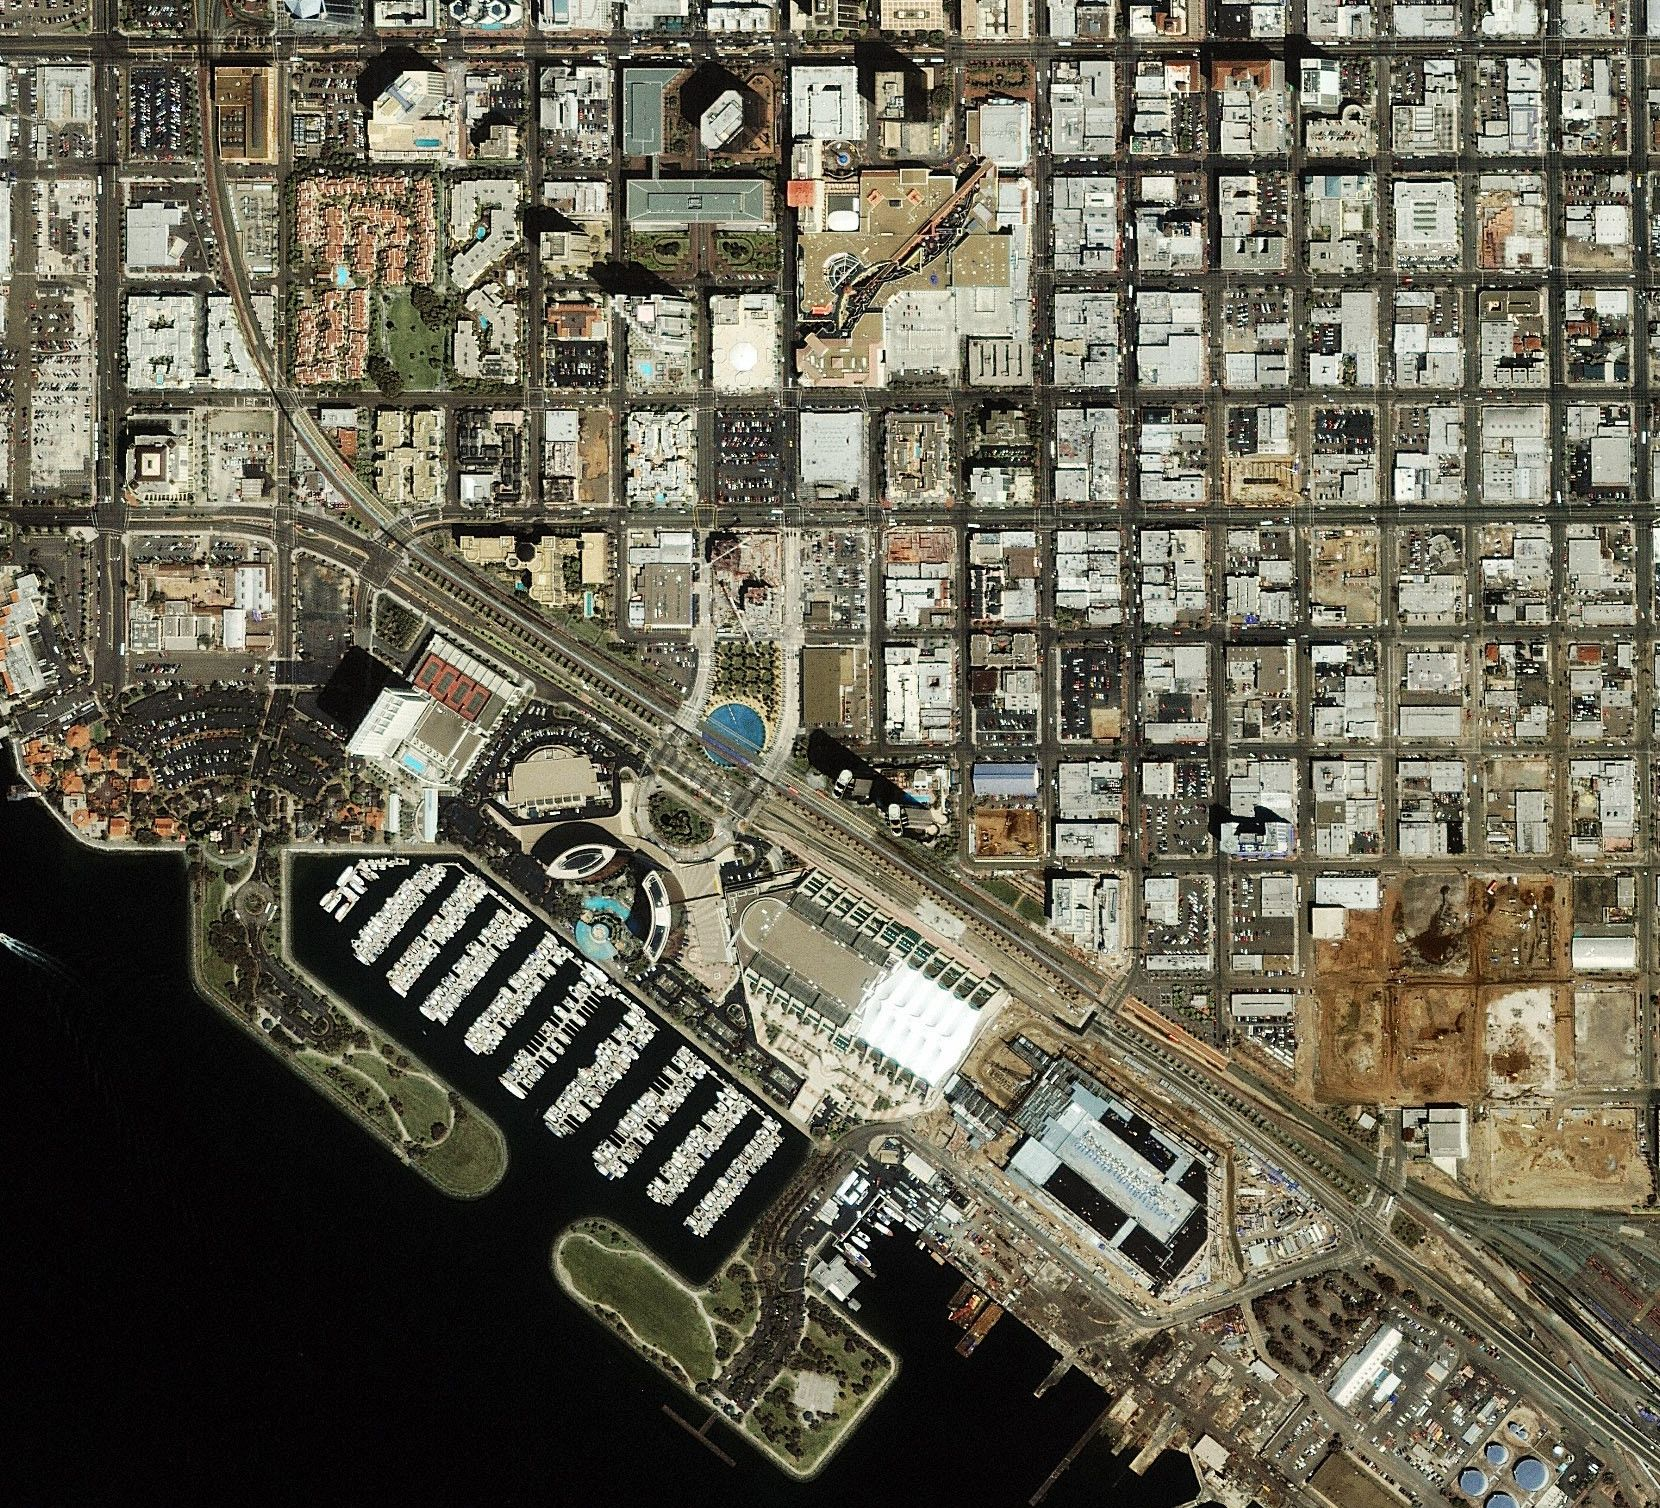
\includegraphics[scale=0.25]{resolution_image.jpg}
\caption{Image satellite en très haute résolution}
\end{figure}

\par
\underline{Valeur des pixels :}
\par 

Chaque pixel d’une image a une valeur. Cette valeur correspond à l’intensité du rayonnement réfléchi par l’objet observé dans la gamme de longueur d’ondes auxquelles le capteur est sensible. \cite{ref3}

La valeur du pixel varie de 0 (= noir) à 255 (= blanc). Donc, il y a 256 possibilités, ce qui correspond à 1 octet. Cela représente la quantité de rayonnement détectée par un capteur, allant du minimum au maximum. Le nombre de niveaux donne une indication quant à la précision de la mesure : plus il y a de niveaux (donc plus il y a de bits), plus détaillée sera la mesure et donc plus précise sera la mesure de la variation du rayonnement.

\begin{figure}[h]
\centering
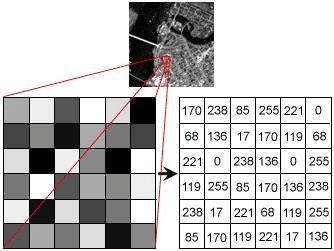
\includegraphics[scale=1.2]{pixel_values.png}
\caption{Les valeurs des pixels}
\end{figure}

\par
En observation de la Terre on peut exploiter :
\begin{mylist}
\item
des ondes émises par le soleil puis réfléchies par la surface de la Terre et enregistrées par un capteur placé sur un satellite.
\item
des ondes émises par un émetteur artificiel placé sur le satellite puis réfléchies par la surface de la Terre et enregistrées par un capteur placé sur ce même satellite.
\end{mylist}

Dans le premier cas on parle d'\textbf{images optiques} (télédétection passive), dans le second cas d'\textbf{images radar} (télédétection active).

\begin{figure}[h]
\centering
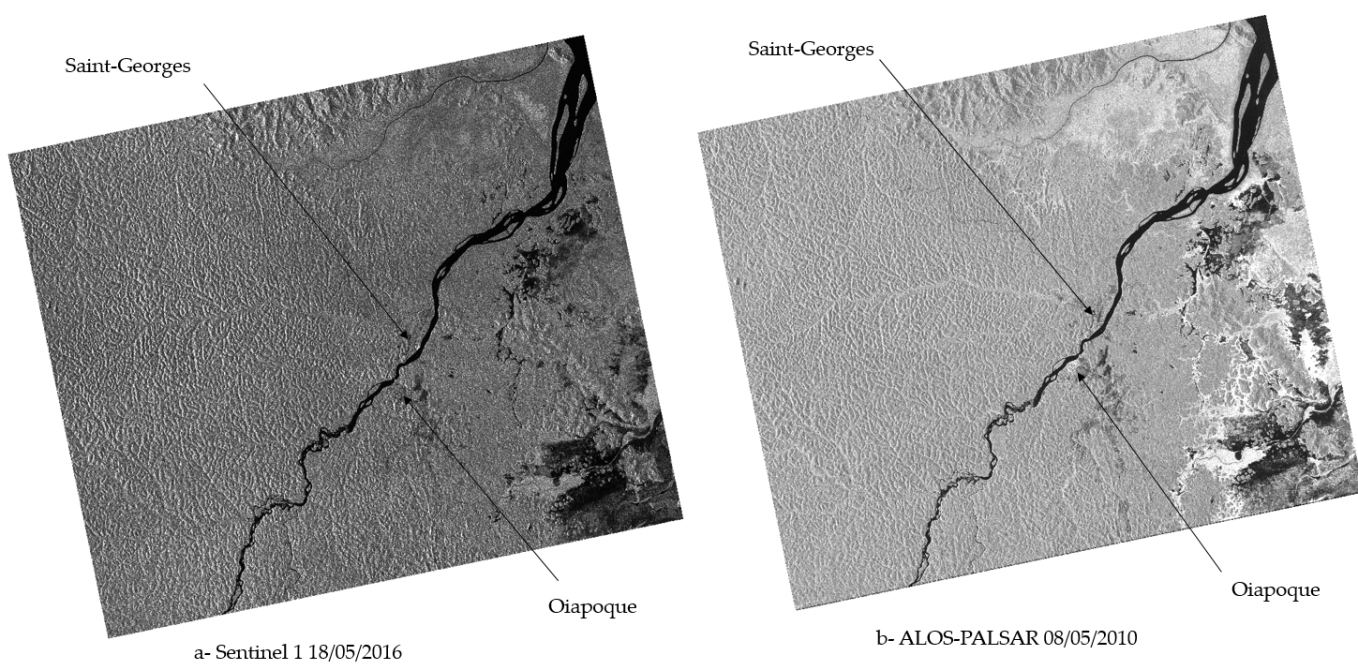
\includegraphics[scale=0.3]{image_radar.png}
\caption{Exemple d'image radar prise par le sattellite Sentinel-1 et ALOS/PALSAR}
\end{figure}

\par
La télédétection radar présente l’avantage de s’affranchir des contraintes de couverture nuageuse : les ondes émises par les satellites traversent les nuages pouvoir acquérir des images de jour comme de nuit. En revanche, leur exploitation pour l’observation de la Terre est moins intuitive quel les images optique, ainsi différents domaines spectraux sont exploité (longueurs d’onde du visible à l’infrarouge).\cite{ref4} \\ \\ \\



\subsection{Les satellites au service de l'agriculture}

Dans le domaine de l'agriculture, les satellites d'observation de la Terre sont utilisés pour une très grande variété d’applications et de services, comme la surveillance des cultures, le contrôle des surfaces et de l'occupation des sols, l'irrigation et la des gestion des cultures en engrais et produits phytosanitaires. Ils sont également utilisés pour suivre la production d'herbe tout au long de la saison culturale.  \cite{satt}


\begin{figure}[h]
\centering
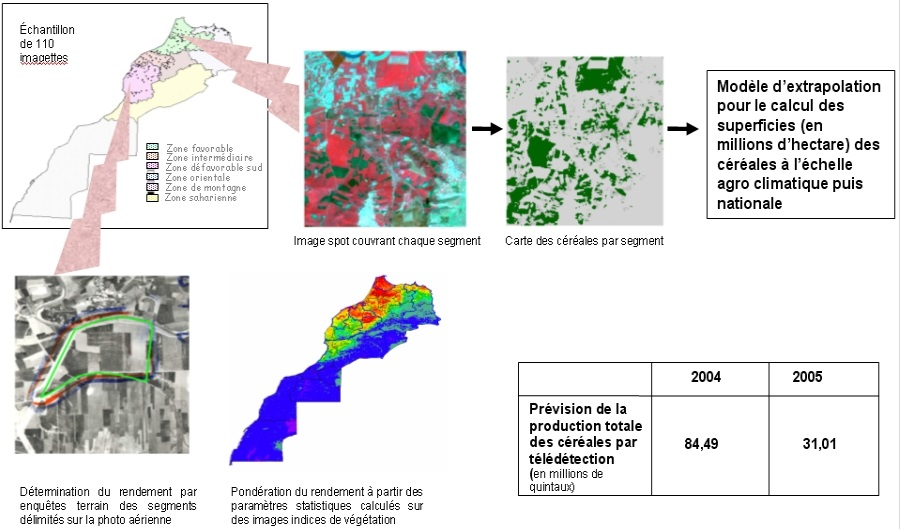
\includegraphics[scale=0.65]{prev.jpg}
\caption{Prévision de la production des céréales à l'échelle nationale}
\end{figure}

L'intérêt d'utiliser des satellites s'explique par leur capacité à  fournir des images multi spectrales de très bonne résolution. Ces images reçues dans plusieurs longueurs d'onde permettent d'estimer des paramètres biophysiques à partir des pixels de l'image que l'on mesure dans plusieurs couleurs de façon à caractériser l'état de la plante.
\par
Ce type d'image a supplanté les systèmes antérieurs en démontrant qu'il pouvait prendre en compte l'état réel des cultures et de la croissance de la végétation à l'intérieur des parcelles à différents stades de la pousse.

\chapter{Analyse du sujet}
\section{Crop Mapping}
\subsection{Définition}
C’est une technique en agriculture qui utilise des données GPS pour analyser des variables telles que le rendement des cultures et la teneur en eau dans un champ donné. Il a été développé dans les années 1990 et utilise une combinaison de technologie GPS et de capteurs physiques, tels que des compteurs de vitesse , pour suivre les rendements des cultures, la vitesse de l'élévateur à grains et combiner la vitesse.
\par
Ces données produisent une carte des rendements qui peut être utilisée pour comparer la distribution des rendements dans le champ d'une année à l'autre. Cela permet aux agriculteurs de déterminer les zones du champ qui, par exemple, peuvent avoir besoin d'être plus fortement irriguées ou qui ne produisent aucune récolte. Il permet également aux agriculteurs de montrer les effets d'un changement dans les techniques de gestion des champs, d'élaborer des stratégies nutritionnelles pour leurs champs et d'enregistrer le rendement des cultures à utiliser pour obtenir des prêts ou des locataires.

\subsection{Les méthodes de Crop Mapping}

Il y a plusieurs méthodes de Crop Mapping dont:

\subsubsection{La télédétection (remote sensing from space)}
La télédétection offre une méthode sûre et efficace de cueillette d'information dans le but de cartographier le type et de calculer la superficie des cultures.
Les micro-ondes sont sensibles à l'alignement, la structure et la quantité d'eau présente dans les plantes et dans le sol, et peuvent fournir de l'information complémentaire aux données optiques. 

\par
Les résultats de l'interprétation des données de télédétection peuvent être intégrés dans un système d'information géographique (SIG) et dans un système de gestion des cultures, et peuvent aussi être combinés à des données auxiliaires pour fournir de l'information sur les droits de propriété, les pratiques de gestion, etc. \cite{cropmapp}\\ \\ \\

\begin{figure}[h]
\centering
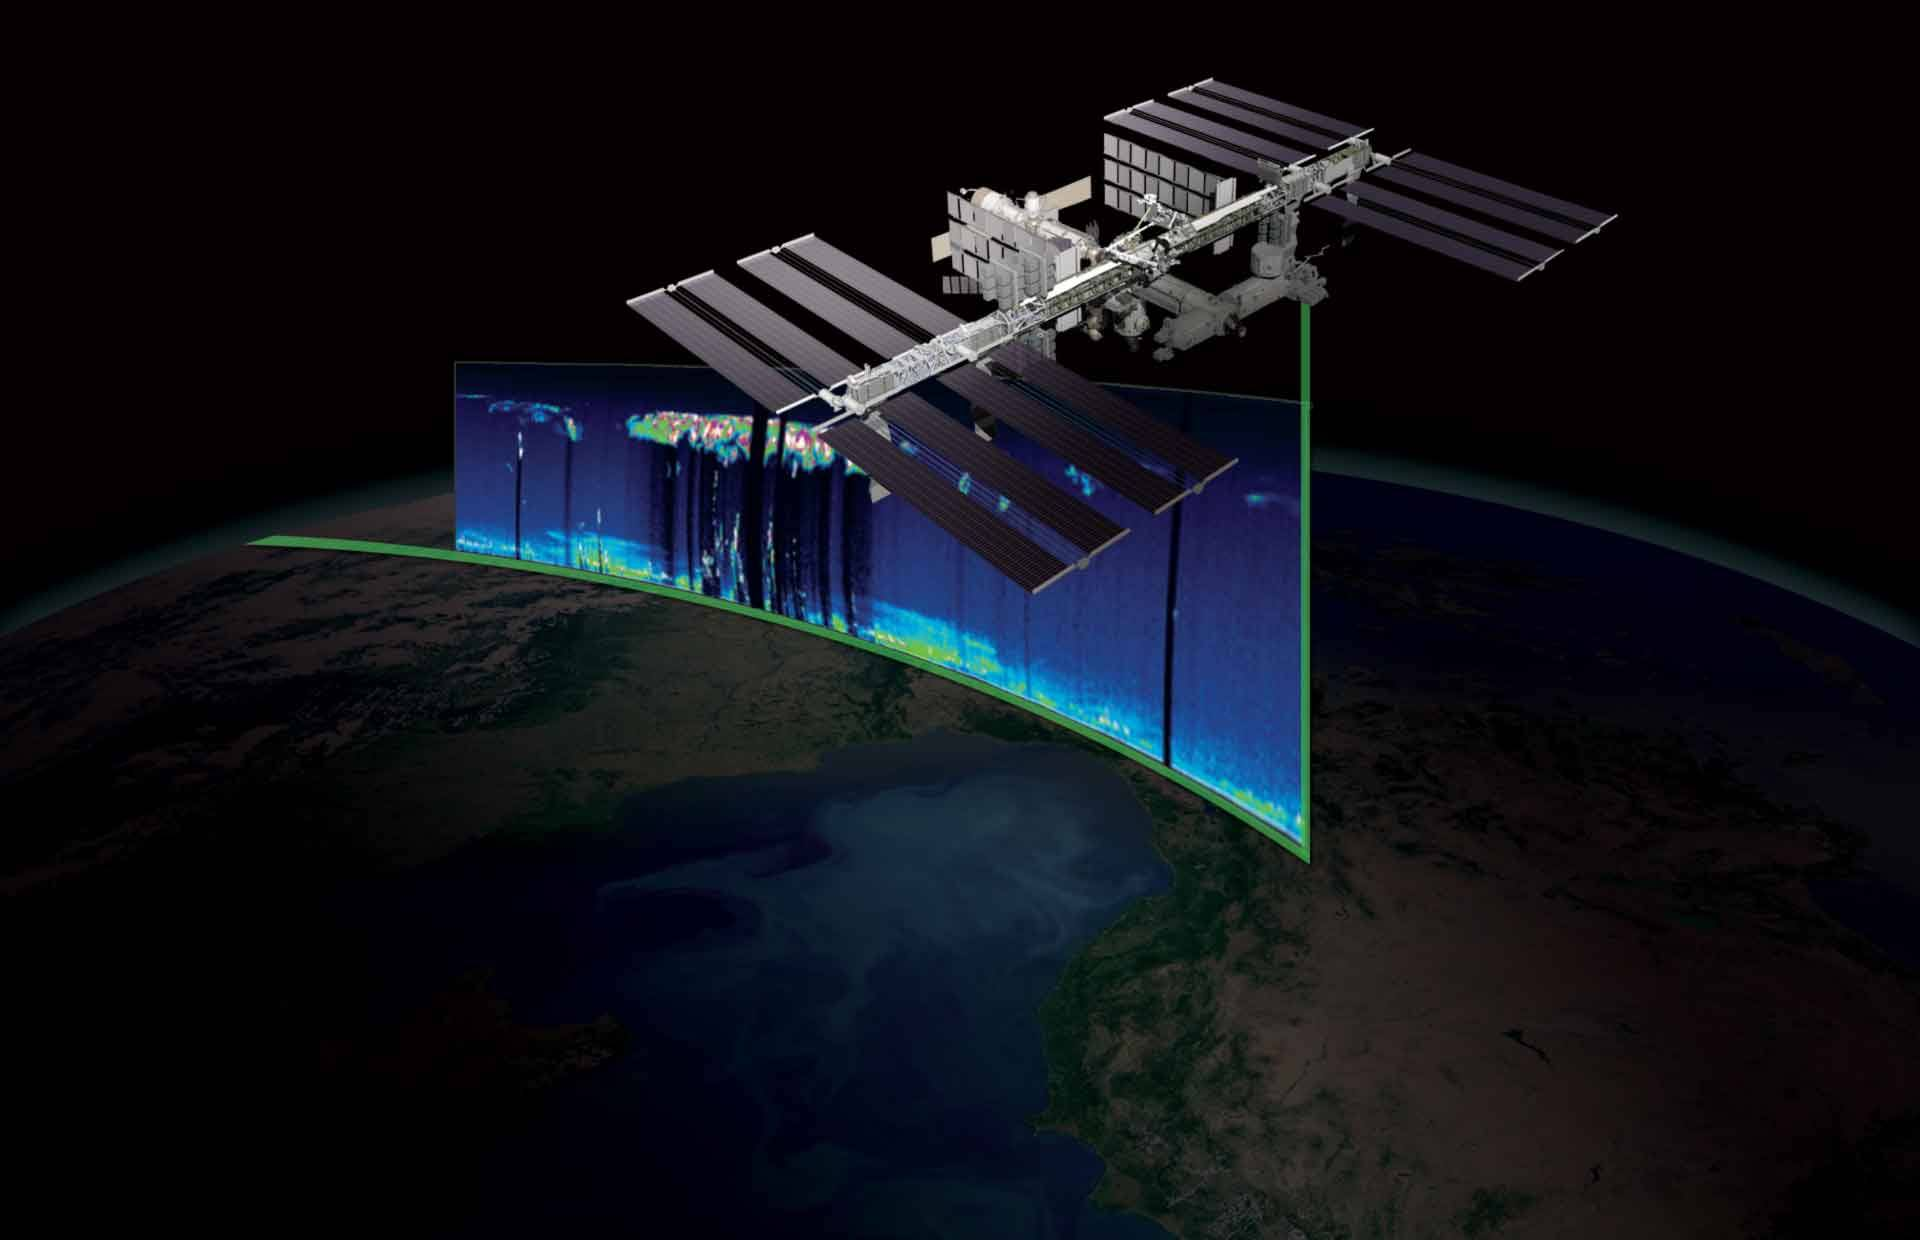
\includegraphics[scale=0.2]{tele.jpg}
\caption{La télédétection par satellite}
\end{figure}

\subsubsection{MODIS (Moderate Resolution Imaging Spectroradiometer)}
MODIS est un instrument clé à bord des satellites Terra et Aqua qui sont en orbite de la terre et qui visualise la totalité de sa surface tous les 1 à 2 jours, acquérant des données dans 36 bandes spectrales.

\begin{figure}[h]
\centering
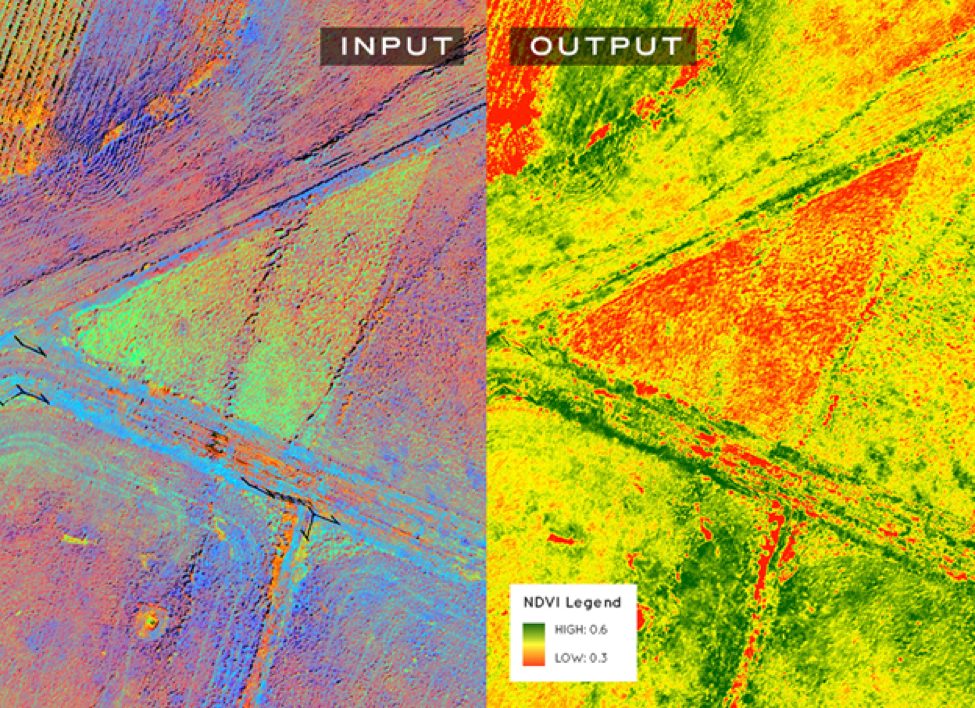
\includegraphics[scale=0.35]{modis.png}
\caption{Une comparaison Input/Output par la méthode MODIS}
\end{figure}

MODIS présente deux indices de végétation (NDVI et EVI) qui fournissent des comparaisons spatiales et temporelles des différentes surfaces à couvert végétale et foliaire, le NDVI (normalized difference vegetation index) assure la continuité de la série temporelle pour des applications historiques et climatiques tandis que le EVI minimise les variations de la canopée et améliore la sensibilité aux conditions de végétation dense.
Ces deux indices caractérisent plus efficacement la gamme mondiale des états et des processus de végétation. \cite{modis}

\subsubsection{Deep Learning Classification}
Le Deep Learning (DL) est une technique de pointe puissante pour le traitement d'image, y compris les images de télédétection (remote sensing images). 
Pour cibler la couverture des sols et la classification des types de cultures à partir d'images satellites multi-temporelles et multi-sources, une architecture DL à plusieurs niveaux solide doit être disposer. 
Le pilier de cette architecture est un réseau neuronal qui est utilisé pour la segmentation des images optiques et la restauration des données manquantes en raison des nuages et des ombres. \cite{deeplearning}

L’avantage de cette méthode est d’étudier des modèles de deep learning/machine learning pour la « crop classification » qui fournissent une segmentation basée sur les pixels d'une zone d'inspection pendant une période donnée. Pour obtenir de meilleurs résultats, il est préférable d’utiliser des modèles existant et de sélectionner ceux les mieux adaptés à la situation. Et pour mieux de flexibilité, il faut ajuster les modèles pré-formés par transfert learning à de nouvelles données comme de nouveaux domaines avec de nouvelles particularités, cultures...

Un autre avantage est le potentiel d'améliorer considérablement la précision d'un modèle avec plus de données réelles recueillies au sol de la région étudié en utilisant des données spécifiques. Cependant, il est possible d'obtenir de meilleurs résultats avec l'ensemble de données de formation (training data set) plus spécifiques.

\begin{figure}[H]
\centering
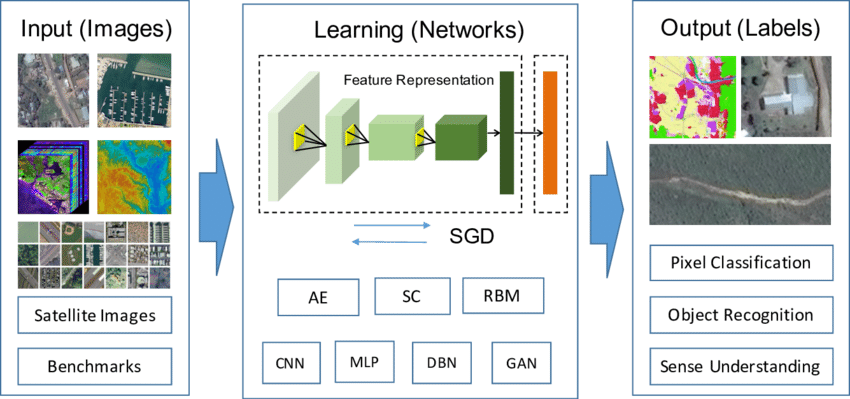
\includegraphics[scale=0.5]{deep.png}
\caption{Le processus de Deep Learning}
\end{figure}

\subsection{Outils pour le Crop Mapping}

On a essayé de faire une comparaison entre les outils les plus populaires dans le domaine du Crop Mapping :

{\setlength{\tabulinesep}{3pt}
\begin{tabu}{|c|c|c|c|c|c|c|}
\hline
\diagbox{caractéristiques}{L'outil}&\href{https://www.harrisgeospatial.com/Software-Technology/ENVI}{ENVI}&\href{https://groundwork.azavea.com}{QGIS}&\href{https://www.arcgis.com/index.html}{ArcGIS}&\href{https://cmapsconnect.com/}{CMaps}&\href{https://clarklabs.org/terrset/}{TerrSet}&\href{https://groundwork.azavea.com/}{Groundwork}\\
\hline
Open Source & - & + & - & - & - & -\\
\hline
Imagerie 3D & - & + & + & - & - & -\\
\hline
Géocodage & - & + & + & + & + & -\\
\hline
Exportation d'images & + & + & + & - & + & +\\
\hline
Internet Mapping & + & - & + & + & - & -\\
\hline
L'interopérabilité & - & + & + & + & - & -\\
\hline
Étiquetage & + & + & + & - & - & +\\
\hline
Création de carte & + & + & + & + & + & +\\
\hline
Partage de carte & - & - & + & + & - & -\\
\hline
\end{tabu}}\\


\subsubsection{Au niveau des algorithmes :}


ENVI incorpore de nombreux algorithmes de fusion d'images bien connus (HSV transformation/Gram-Schmidt Spectral Sharpening, PC Spectral Sharpening/...) entre autres transformations de bande (Veg. Index calculation/ Tasseled Cap Transformation/ ...). Le côté positif est le fait que vous pouvez facilement programmer ENVI avec IDL pour effectuer des travaux de traitement par lots (beaucoup de données) ou créer un programme IDL autonome pour une autre transformation non déjà incluse dans ENVI.\\

QGIS est principalement conçu pour fonctionner avec des données vectorielles de type GIS (Geographic Information System), il prend en charge de nombreux formats d'images raster (svg, jpg, png, tif, ...) via les bibliothèques open source GDAL et GRASS.\\

Enfin, il existe de nombreux codes spécifiques au format pour plusieurs langages (Python, C, Java, etc.) qui vous permettront de lire les données et d'appliquer les transformations nécessaires.\\

\subsubsection{Test de l'outil QGIS :}
QGIS utilise Orfeo ToolBox (OTB) qui est une bibliothèque d’algorithmes de traitement d’image. OTB est basée sur la bibliothèque de traitement d’images médicales et fournit des fonctionnalités dédiées aux traitements d’images de télédétection ou pour les images de haute résolution spatiale. Les algorithmes dédiés aux images de grandes résolutions optiques (Pleiades, SPOT, QuickBird, WorldView, Landsat, Ikonos), aux capteurs hyperspectraux sensors (Hyperion) ou aux radars à synthèse d’ouverture (TerraSarX, ERS, Palsar) sont disponibles.
\begin{figure}[ht]
\centering
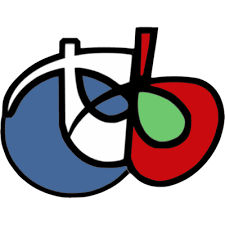
\includegraphics[scale=0.5]{orfeo.png}
\caption{La bibliothèque Orfeo ToolBox (OTB)}
\end{figure}

Le module "otb" permet l'utilisation de la bibliothèque de calcul numérique haute performance "TensorFlow" . L'API C ++ de TensorFlow est utilisée pour exécuter des sessions tensorflow à l' intérieur de filtres conformes au mécanisme de streaming d'ITK et OTB, ce qui signifie qu'il n'y a pas de limitation sur la taille des images à traiter.


Voici un exemple de segmentation qu'offre QGIS :
\begin{figure}[ht]
\centering
\noindent
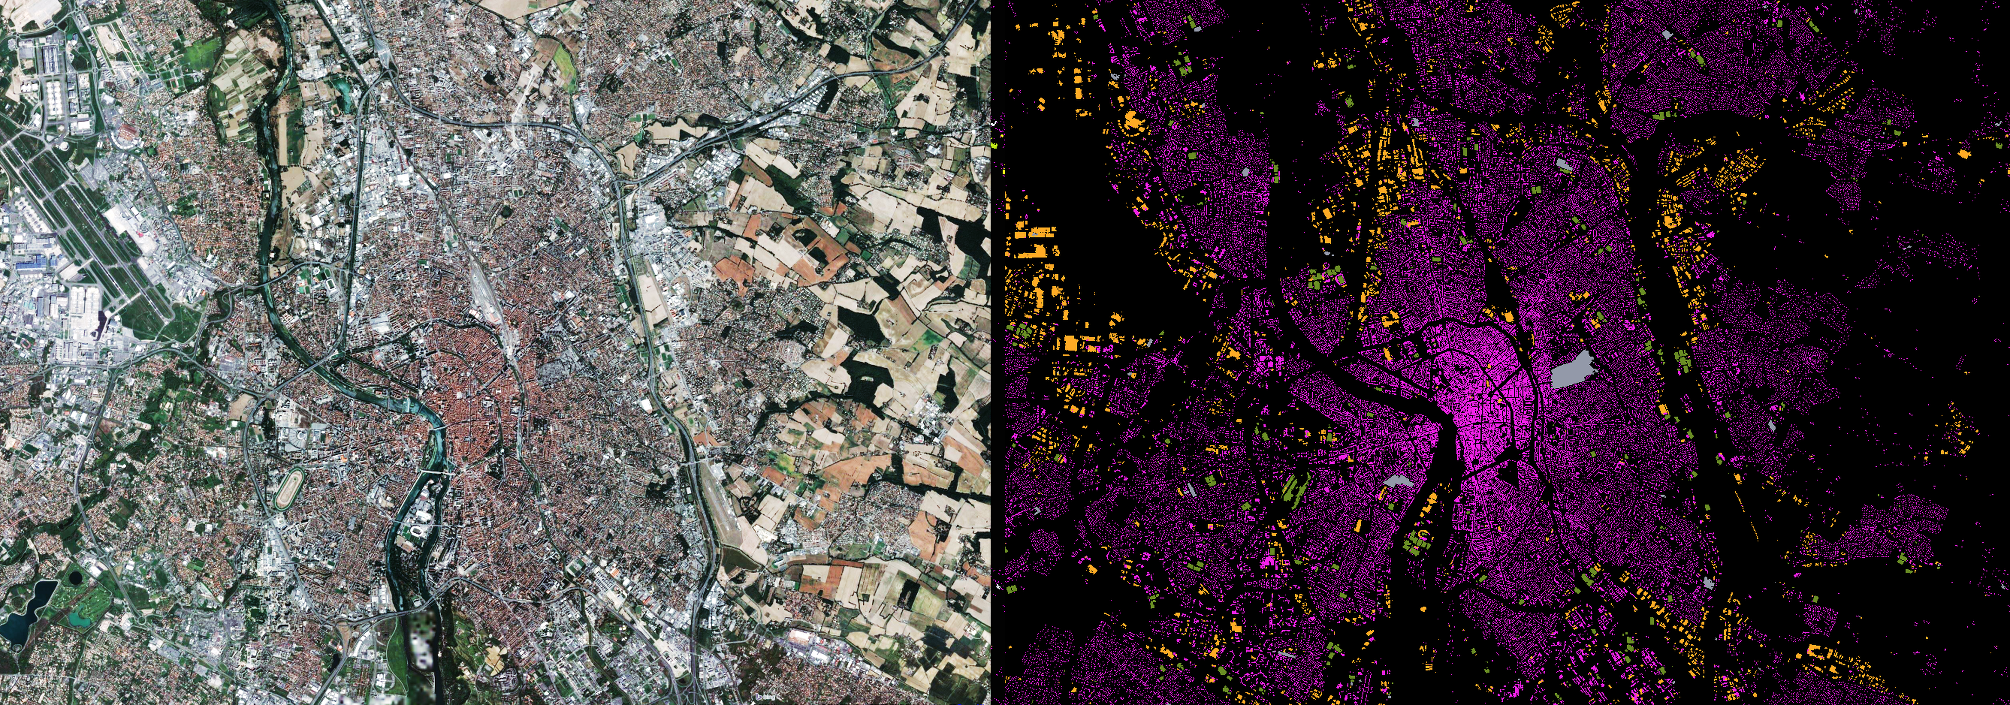
\includegraphics[width=1\textwidth]{test_segmentation.png}
\caption{Segmentation avec QGIS}
\end{figure}

\newpage
\subsubsection{Test de l'outil Groundwork :}
\begin{figure}[h]
\centering

\includegraphics[scale=0.4]{Groundwork.png}
\caption{Groundwork logo}
\end{figure}

On a testé l'outil GroundWork de la compagnie azavea qui est en charge à la réalisation des modèles personalisé de machine learning qui analyse les images de drones et de satellites.
Cette outil qui est gratuit permet la création d'une "training data set" d'image géospatiale en implémentant une machine learning.
\par
La création du projet est comme ce qui suit : on determine d'abord le type du projet, c'est à dire soit détection d'objet, segmentation sémantique ou classification d'image, ensuite, on entre l'url de l'image qu'on veut ségmenter, puis on spécifie ce qu'on doit ségmenter (surface verte, l'eau, le sol ...) ainsi avec son processus de machine learning il nous ségmente notre image avec les classes que nous avons définis.
A la fin, on exporte notre image avec les étiquettes, mais aussi des données qu'on peut traiter avec pySTAC qui est une bibliothèque de python crée par la même compagnie.

\begin{figure}[h]
\centering
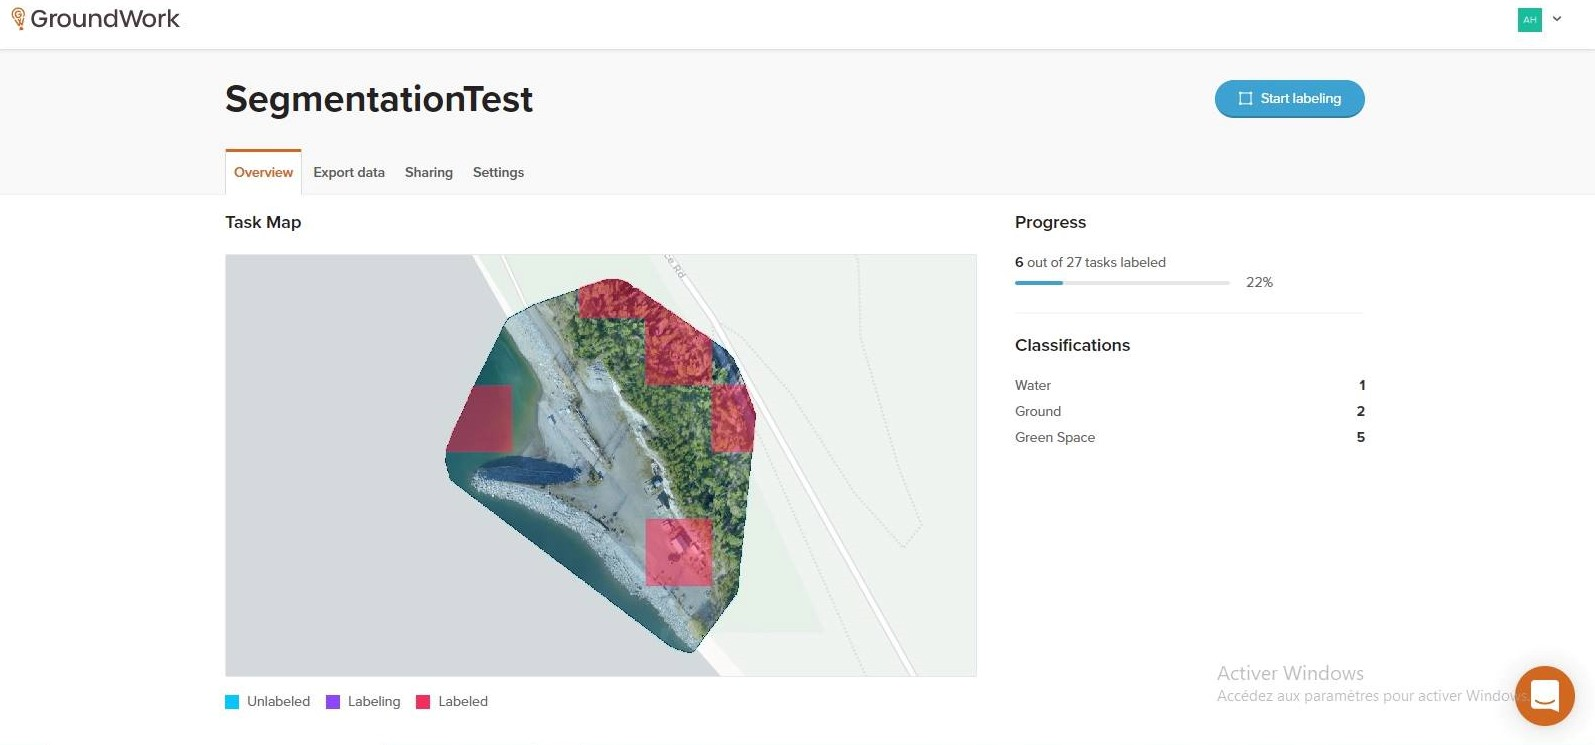
\includegraphics[scale=0.4]{groundwork_screen1.jpg}
\caption{Groundwork analysant l'image partie par partie}
\end{figure}

\begin{figure}[h]
\centering
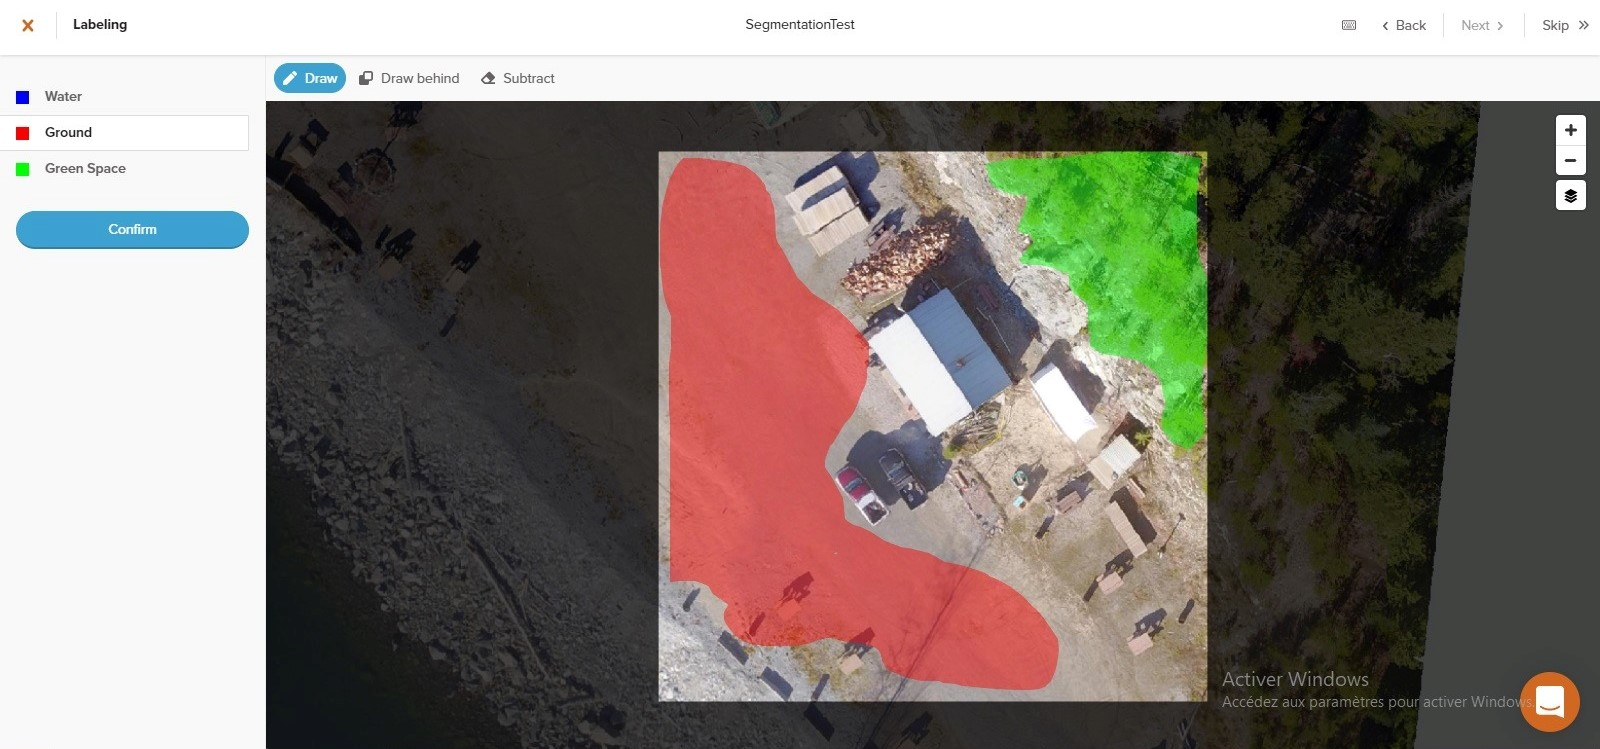
\includegraphics[scale=0.4]{groundwork_screen2.jpg}
\caption{Résultat d'une fragmentation d'un image avec des étiquettes}
\end{figure}

%Deuxième partie ____________________________________________________%

\part{Réalisation}

\chapter{Ségmentation et application des filtres}

\section{Algorithmes de segmentation}

\subsection{Support Vector Machine (SVM)}

\subsubsection{Définition}
En Machine Learning, les machines à vecteurs de support (SVM) sont des modèles d'apprentissage supervisé avec des algorithmes d'apprentissage associés destinées à résoudre des problèmes de discrimination et de régression. 
\par
Un modèle SVM est une représentation des exemples sous forme de points
dans l'espace, cartographiée de manière à ce que les exemples des catégories distinctes soient divisés par un espace clair aussi large que possible. De nouveaux exemples sont ensuite mappés dans ce même espace et devraient appartenir à une catégorie en fonction du côté de l'écart sur lequel ils se trouvent.
\begin{figure}[h]
\centering
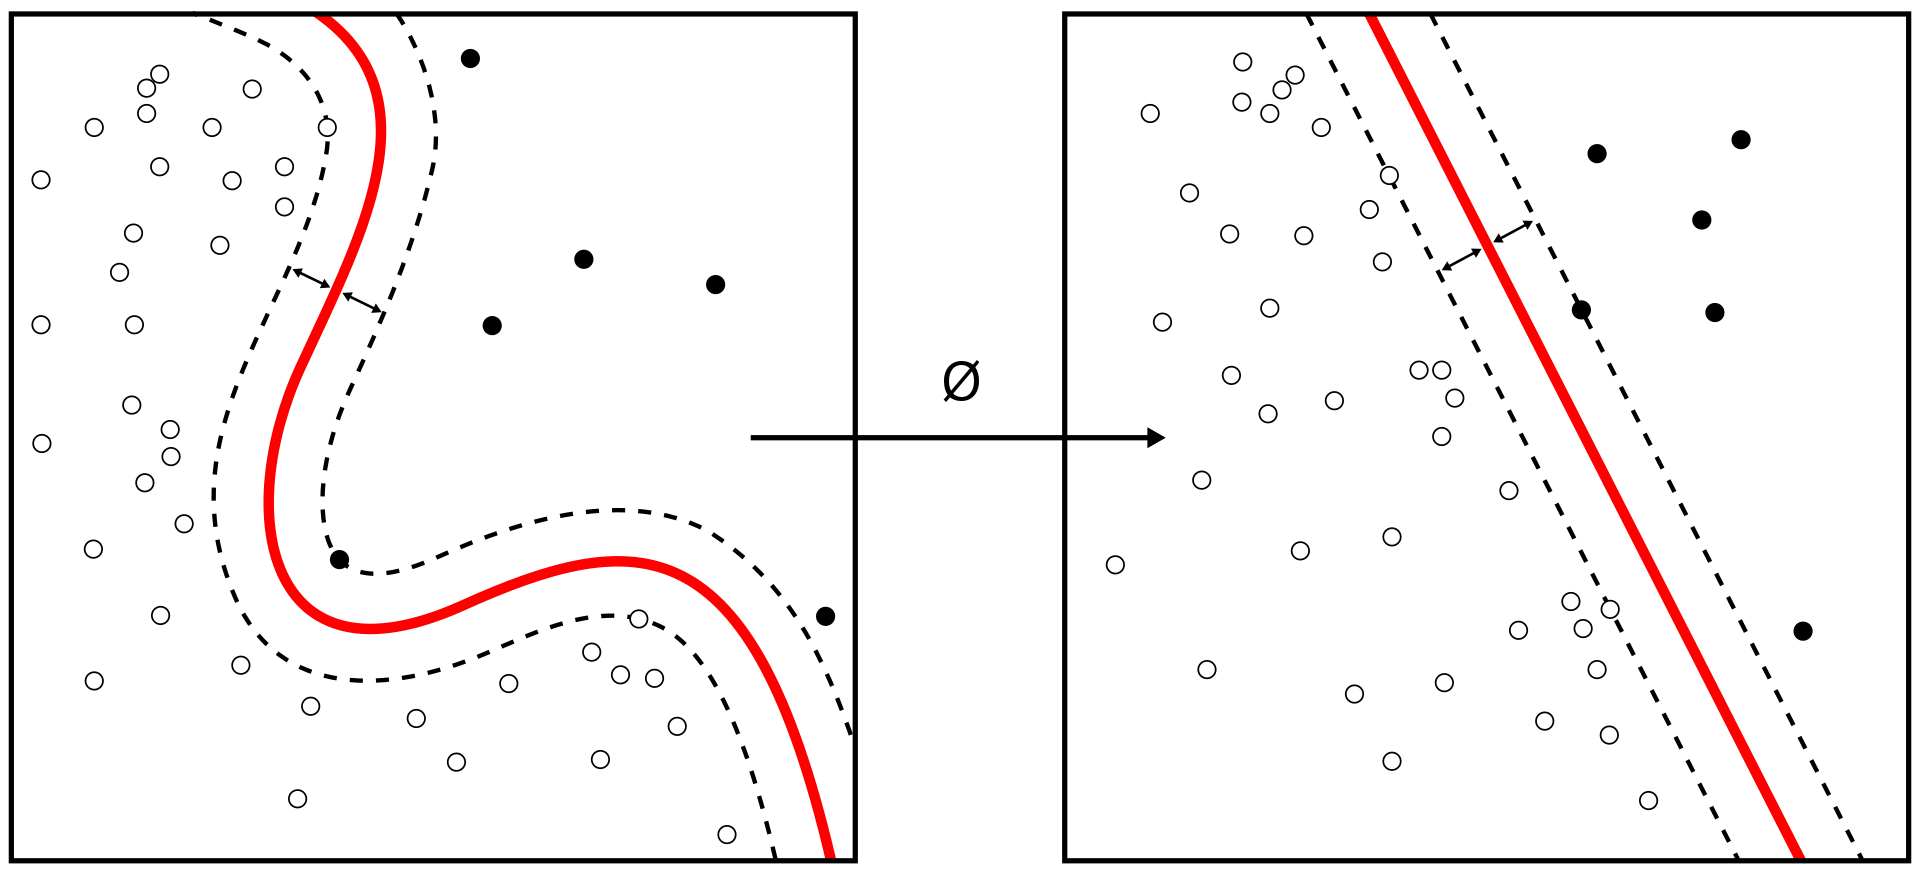
\includegraphics[scale=0.2]{svm.png}
\caption{Division de l'espace par SVM}
\end{figure}

\par
Les SVM ont été appliqués à de très nombreux domaines (bio-informatique, recherche d'information, vision par ordinateur, finance1…). Selon les données, la performance des machines à vecteurs de support est de même ordre, ou même supérieure, à celle d'un réseau de neurones ou d'un modèle de mélanges gaussiens.

\subsubsection{SVM dans python}
Dans Scikit-learn, les SVM sont implémentées dans le module "sklearn.svm".
Scikit-Learn contient la bibliothèque svm, qui contient des classes intégrées pour différents algorithmes SVM. 
\par
Nous avons effectuer une tâche de classification supervisé sur image sattelite d'une culture entre la région d'Assilah et Larache, nous utiliserons la classe de classificateur de vecteur de support, qui se nomme 'SVC' dans la bibliothèque svm de Scikit-Learn.
\par
Cette classe prend plusieurs paramètres qui sont en ralations avec des formules mathématiques correspondantes à SVM, et qui peuvent affecter le degré de netteté de la ségmentation.
\par
Voici un exemple d'une ségmentation en définissant trois classes sur l'image originale : 

\begin{figure}[h]
\centering
\hspace*{-0.5in}
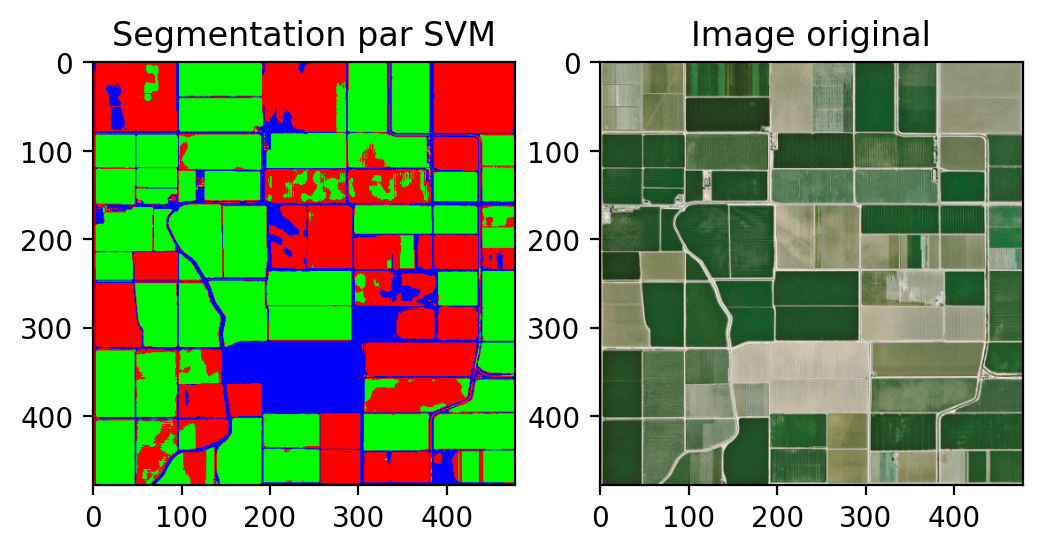
\includegraphics[scale=0.9]{classification.png}
\caption{Classification par SVM}
\end{figure}

\noindent Les classes sont les suivantes : 

\begin{mylist}
\item La partie verte : végétation.
\item La partie rouge : terre fertilisée.
\item La partie bleu : terre rocheuse.
\end{mylist}

\subsection{K-means algorithm}


K-Means Clustering est un algorithme de machine learning non supervisé. Contrairement aux algorithmes traditionnels de machine learning supervisé, K-Means tente de classer les données sans avoir d'abord été formé avec des données étiquetées. Une fois l'algorithme exécuté et les groupes définis, toutes les nouvelles données peuvent être facilement attribuées au groupe le plus pertinent.
\par 
Parmi les applications réelles de k-means on trouve : le profiling, la segmentation du marché, les moteurs de recherche, l'astronomie ...\cite{k-means}

\par
Pour son application on a utilisé la même image précédente et on a définie trois cluster pour la ségmentation voice le résultat : 

\begin{figure}[ht]
\centering
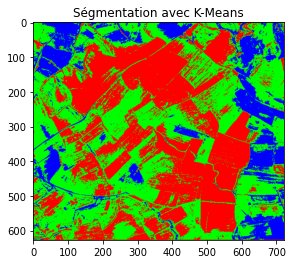
\includegraphics[scale=0.9]{kmeans.png}
\caption{Segmentation avec K-Means}
\end{figure}

\subsection{Multi-Otsu threshold}
Le seuil multi-Otsu est un algorithme de seuillage utilisé pour séparer les pixels d'une image d'entrée en plusieurs classes différentes, chacune obtenue en fonction de l'intensité des niveaux de gris dans l'image.
Multi-Otsu calcule plusieurs seuils, déterminés par le nombre de classes. Le nombre de classes par défaut est 3: pour obtenir trois classes, l'algorithme renvoie deux valeurs de seuil.

\begin{figure}[ht]
\centering
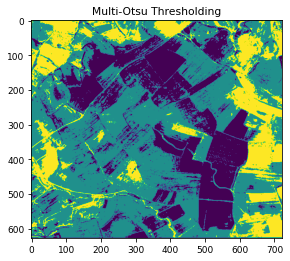
\includegraphics[scale=0.9]{osupng.png}
\caption{Segmentation avec multi-Otsu threshold}
\end{figure}

\section{Comparaison des méthodes de détection des contours\cite{comparaison}}
Le contour c’est la zone où il existe des différences extrêmes dans les intensités du pixel indique généralement un bord d'un objet.
Nous mettrons en œuvre certaines des méthodes les plus utilisées et utiliserons également les méthodes d'Open CV et de PIL.
\noindent Nous comparerons les méthodes suivantes:
\begin{mylist}
\item Détecteur de contour Sobel
\item Détecteur de contour Prewitt
\item Détecteur de contour Canny
\end{mylist}

\subsection{Opérateur Sobel}
Sobel est un opérateur très courant pour détecter les bords d'une image, qui est une approximation d'une dérivée d'une image. Il est séparé dans les directions 'y' et 'x'. Ici, nous utilisons une matrice de noyau 3 * 3, une pour chaque direction 'x' et 'y'. Le gradient pour la direction 'x' a des nombres négatifs à gauche et des nombres positifs à droite et nous préservons les pixels centraux. De même, le gradient pour la direction 'y' a des nombres négatifs en bas et des nombres positifs en haut .

\begin{figure}[H]
\centering
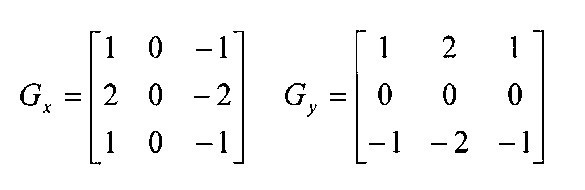
\includegraphics[scale=0.9]{sobel_masque.jpg}
\caption{Le masque de Sobel}
\end{figure}

Voici le résultat en appliquant le filtre de Sobel à l'image original :

\begin{figure}[H]
\centering
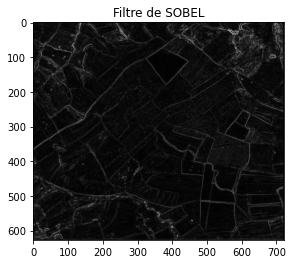
\includegraphics[scale=0.9]{sobel_result.png}
\caption{Filtre de Sobel appliqué à l'image originale}
\end{figure}


\subsection{Opérateur de Prewitt}
L'opérateur de Prewitt est similaire à l'opérateur de Sobel, il est utilisé pour détecter les contours verticaux et horizontaux dans les images. Cependant, contrairement au Sobel, cet opérateur ne met pas l'accent sur les pixels les plus proches du centre du masque.

\begin{figure}[H]
\centering
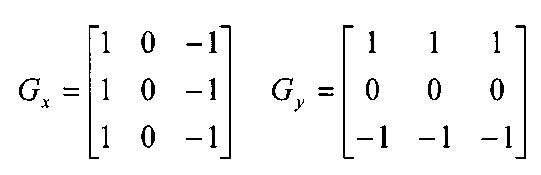
\includegraphics[scale=0.9]{prewit_masque.png}
\caption{Masque de prewitt}
\end{figure}

Au niveau du code, la seule différence est le masque.
Le résultat est le suivant : 
\begin{figure}[H]
\centering
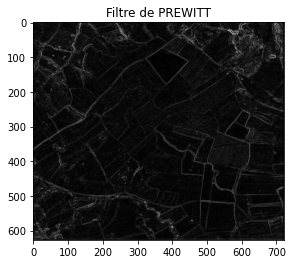
\includegraphics[scale=0.9]{prewitt_result.png}
\caption{Application du filtre de Prewitt}
\end{figure}

\subsection{Opérateur Canny}
Le détecteur de contour Canny est probablement la méthode la plus utilisée et la plus efficace, c'est une méthode de détection de contour beaucoup plus complexe que celles décrites ci-dessus.
\noindent Les étapes de cette méthode sont les suivantes :
\begin{enumerate}
    \item Lissage de l'image avec un filtre gaussien pour réduire le bruit.
    \item Le calcul du gradient en utilisant l'un des opérateurs de gradient Sobel ou Prewitt.
    \item Extraction des points de contour: suppression non maximale.
    \item Liaison et seuillage: hystérésis
\end{enumerate}

Après les deux premières étapes, il faut également calculer l'orientation des gradients «thêta = arctan (Gy / Gx)». Gy et Gx sont respectivement la direction x du gradient et la direction y.
Parlons maintenant de la suppression non maximale et de ce qu'elle fait. Dans cette étape, nous essayons de relier la direction des contours à une direction qui peut être tracée le long des contours en fonction des forces de gradient et des directions des contours précédemment calculées. À chaque emplacement de pixel, nous avons quatre directions possibles. Nous vérifions toutes les directions si le gradient est maximum à ce point. Les valeurs de pixels perpendiculaires sont comparées à la valeur dans la direction du contour. Si leur valeur est inférieure au pixel sur le contour, ils sont supprimés. Après cette étape, nous obtiendrons des contours minces cassés qui doivent être réparés, alors passons à l'étape suivante.
L'hystérésis est un moyen de relier les lignes brisées produites à l'étape précédente. Cela se fait en itérant sur les pixels et en vérifiant si le pixel actuel est un contour. S'il s'agit d'un contour, vérifiez les environs pour les contours. S'ils ont la même direction, nous les marquons comme pixel de contour. Nous utilisons également 2 seuils, un haut et un bas. Si les pixels sont supérieurs au seuil inférieur, ils sont marqués comme un contour. Ensuite, les pixels supérieurs au seuil inférieur et également supérieurs au seuil élevé sont également sélectionnés comme pixels à fort contour. Quand il n'y a plus de changements à l'image, nous nous arrêtons.

\begin{figure}[H]
\centering
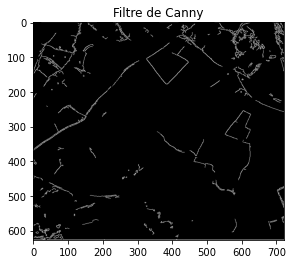
\includegraphics[scale=0.78]{filtre de canny.png}
\caption{Masque de canny}
\end{figure}

















%Bibliographie_______________________________________________________

\begin{thebibliography}{9}

\bibitem{frag}
Agriculture et Biodiversité en Bretagne\\
\textit{Freagmentation du parcellaire}. \\
\url{http://www.agriculturebiodiversite.fr/ameliorer-la-biodiversite/amenager-son-exploitation/fragmentation-du-parcellaire.html}

\bibitem{imagesatt}
Les images et les statistiques concernat le Maroc\\
\textit{Centre Royal de Télédétection Spatiale}.\\
\url{https://www.crts.gov.ma/thematiques/agriculture/suivi-d-etat-des-cultures}

\bibitem{agr}
Agriculture en chiffres 2018 (édition 2019)\\
\textit{Ministère de l'Agriculture, de la Pêche Maritime, du Développement Rural et des Eaux et Forêts}\\
\url{http://www.agriculture.gov.ma/pages/publications/agriculture-en-chiffres-2018-edition-2019}

\bibitem{orbite}
Combien de satellite tournent autour de la Terre ?\\
\textit{Céline Deluzarche, Publié le 12/04/2020, FUTURA SCIENCES}\\
\url{https://www.futura-sciences.com/sciences/questions-reponses/satellite-satellites-tournent-autour-terre-7065/}

\bibitem{ref3}
Les informations contenues dans une image, analogique ou digital ?\\
textit{ESA (European Space Agency) eduspace, 2015}\\
\url{https://www.esa.int/SPECIALS/Eduspace_FR/SEM11YR7NWF_0.html?fbclid=IwAR1DA8wJKDujA2pHMdAoyIz54p5T6kFdVWR6EkySLQCe5O98j66p2ob9LSQ}

\bibitem{ref4}
Comprendre une image satellitaire\\
\textit{GéoBretagne Publication de 2016}\\
\url{https://cms.geobretagne.fr/content/comprendre-une-image-satellitaire?fbclid=IwAR1kR644UcZJa0bt_ZamhZt5UldAfCv-Na9Cto6f2yS-5eiIkAgjWaclgc0}

\bibitem{satt} 
Les satellites au service de l'agriculture\\
\textit{Article de Rémy Decourt publié le 4 avril 2011}.\\
\url{https://www.futura-sciences.com/sciences/actualites/astronautique-satellites-service-agriculture-29034/}

\bibitem{cropmapp}
Generating Crop Classification Maps Using AI\\
\textit{David Markowitz, 6 May 2019, Planet Watchers}\\
\url{https://www.planetwatchers.com/generating-crop-classification-maps-using-ai}

\bibitem{modis}
MODIS Vegetation Index Products\\
\textit{Kamel Didan, Moderate Resolution Imaging Spectroradiometer, NASA}\\
\url{https://modis.gsfc.nasa.gov/data/dataprod/mod13.php}

\bibitem{deeplearning}
Deep Learning Classification\\
\textit{ IEEE Geoscience and Remote Sensing Letters ( Volume: 14 , Issue: 5 , May 2017 }\\
\url{https://ieeexplore.ieee.org/abstract/document/7891032?fbclid=IwAR3TiBL273ykf0RpPCORrCK0hayB4ePCgp21eh76O0cBOBMBszCdKtk2E1g}

\bibitem{k-means}
K-means Clustering Python Example\\
\textit{Cory Maklin, Medium, Dec 28/2018}
\url{https://towardsdatascience.com/machine-learning-algorithms-part-9-k-means-example-in-python-f2ad05ed5203}

\bibitem{comparaison}
Comparing Edge Detection Methods\\
\textit{Nike Tsankashvili, 20 Jan 2018, Medium}\\
\url{https://medium.com/@nikatsanka/comparing-edge-detection-methods-638a2919476e}




\end{thebibliography}

\end{document}








